% !TEX TS–program = pdflatexmk

%\documentclass[lucida,biblatex]{sp} % use if you have the Lucida LaTeX fonts
\documentclass{sp}          % default: uses Times font
\usepackage{textcomp}
\usepackage{algorithm}
\usepackage{algpseudocode}
\usepackage{tikz}
\usepackage{tikz-dependency}
\usepackage{gb4e}
\usepackage{amssymb}
\usepackage{pifont}
\usepackage{tipa}
\usetikzlibrary{fit,positioning}
\usepackage{setspace}
\usepackage{color}
\usepackage{bbm}
\usepackage{enumitem}
\usepackage{mathrsfs}  
\usepackage{bbm}


\addbibresource{references.bib}

\usepackage[utf8]{inputenc}

%\linespread{2}


%tables
\usepackage{tabularx}
\usepackage{array}
\usepackage{booktabs}
\usepackage{multirow}
\newcolumntype{L}[1]{>{\raggedright\let\newline\\\arraybackslash\hspace{0pt}}m{#1}}
\newcolumntype{C}[1]{>{\centering\let\newline\\\arraybackslash\hspace{0pt}}m{#1}}
\newcolumntype{R}[1]{>{\raggedleft\let\newline\\\arraybackslash\hspace{0pt}}m{#1}}
\newcommand{\possessivecite}[1]{\textciteauthor{#1}'s (\textciteyear{#1})}

\newcounter{excounter}

%=====================================================================
%========================= preamble material =========================

% Metadata for the PDF output. ASCII-only!
\pdfauthor{Aleeza Yu}
\pdftitle{Listener adaptation to speaker variation in use of uncertainty expressions}
%\pdfkeywords{Full keyword list}

% Optional short title inside square brackets, for the running headers.
% If no short title is given, no title appears in the headers.
\title{Listener adaptation to speaker variation in use of uncertainty expressions}

% Optional short author inside square brackets, for the running headers.
% If no short author is given, no authors print in the headers.
\author{% As many authors as you like, each separated by \AND.
  \spauthor{Replication of adaptation experiment by Sebastian Schuster and Judith Degen
  Aleeza Yu\\ \today}
}

%=====================================================================

\begin{document}

%=====================================================================
%============================ frontmatter ============================

\maketitle

%\begin{abstract}

%\end{abstract}

%\begin{keywords}
%  Keywords (special formatting is fine)
%\end{keywords}

%=====================================================================
%============================ article text ===========================

\section{Introduction}

I am curious to see whether speakers use different expressions of uncertainty and whether listeners adapt to various uncertainty expressions (e.g. probably or could) used by different speakers. During language comprehension, as listeners, we are constantly making predictions of how a speaker’s sentence will unfold, and we learn to adapt to a speaker’s way of speech and make predictions based off of a specific speaker’s mannerisms. In Yildirim et al. 2016, they found that listeners adapt to a speaker’s use of quantifier expressions (e.g. some or many) after being exposed to biasing conditions. I predict similar results and believe that if listeners are exposed to a speaker with a bias to a specific uncertainty expression, listeners will begin to adapt to the speaker’s choice of uncertainty expression and will later be able to make predictions on what the speaker will use in a sentence.

In Schuster’s adaptation experiment, he conducted two studies through experiments and computational modeling: a pre-test experiment and adaptation experiment. The pre-test experiment was used to evaluate whether there was variation in the use of expressions of uncertainty. Participants were shown a scene with a cartoon adult and little girl with a gumball machine and asked to rate the probability of the adult describing the number of gumballs to the little girl using a sentence with a specific uncertainty expression. There were 15 conditions with two out of the six utterances always being shown. Participants distributed 100 points to three sliders: two sliders had the uncertainty expressions and the other one said, “something else.” Each participant saw 3 trials for each of the following percentages:
0\%, 10\%, 25\%, 40\%, 50\%, 60\%, 75\%, 90\%, 100\%. 

The six utterances were:

\begin{itemize}
\item You’ll get a blue/orange one (bare)
\item You might get a blue/orange one (might)
\item You’ll probably get a blue/orange one (probably)
\item I think you’ll get a blue/orange one (think)
\item It looks like you’ll get a blue/orange one (looks like) 
\item You could get a blue/orange one (could) 
\end{itemize}

I was interested in the bare-probably condition, where speakers always saw the two utterances You’ll get a blue/orange one and You’ll probably get a blue/orange one. 

\begin{center}
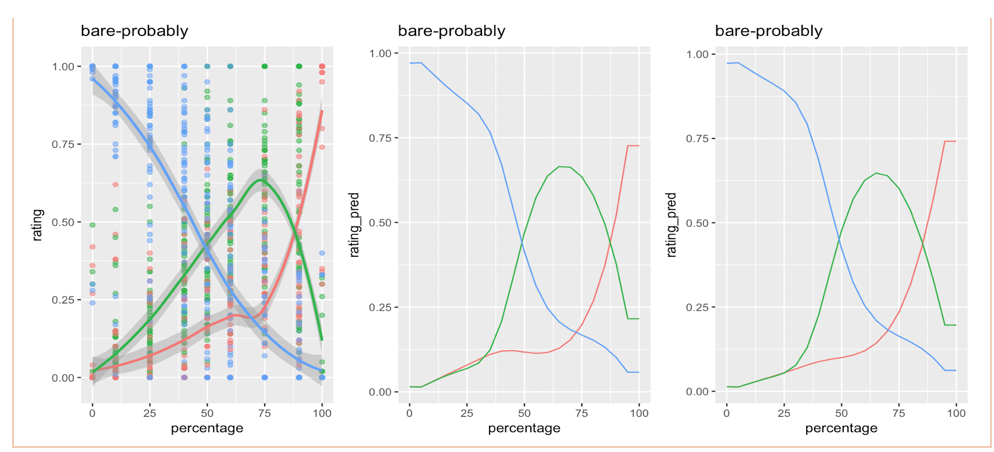
\includegraphics[scale=0.6]{pre-test-bare-probably.png}
\end{center}

As these graphs show, when there is an 85\% chance of getting a blue gumball, some participants rate the bare form higher than probably and vice versa. I chose this condition to study whether listeners adapt to a speaker’s use of an uncertainty expression versus a lack of an uncertainty expression after being exposed to a speaker for some time. 

\subsection{Adaptation experiment}

\subsection{Participants}
A total of 80 participants were recruited via Amazon’s Mechanical Turk. The experiment took about 10-12 minutes to complete. Participants were paid \$1.00 (\$6.00/h).

\subsection{Materials}


Participants first watched 20 scenes in which they saw a child and a gumball machine with different percentages of blue to orange gumballs. Unlike the pre-test experiment where a cartoon adult was used, participants watched a short video in which each trial a man or a woman (speaker gender was randomized across participants) spoke one of the following three utterances.

\begin{itemize}
\item You'll get a blue/orange one (\textsc{bare})
\item You might get a blue/orange one (\textsc{might})
\item You'll probably get a blue/orange one (\textsc{probably})
\end{itemize}

After they were exposed to these 20 scenes, participants were instructed that the child could not see the gumball, therefore the speaker in the video was responsible for telling the child how likely it would be for them to get a blue/orange gumball. Participants were asked to rate how likely they think the speaker is to use the three utterances that are presented below the scene, by distributing 100 points using three sliders.

\begin{center}
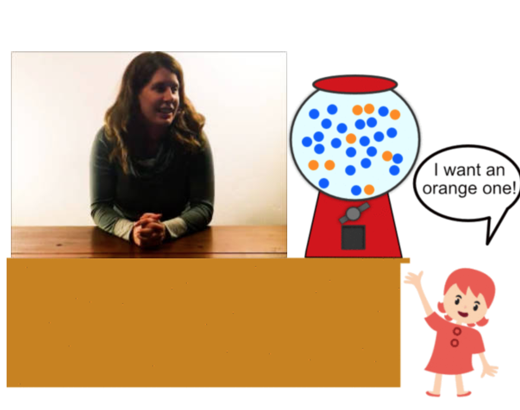
\includegraphics[scale=0.5]{female-condition.png}
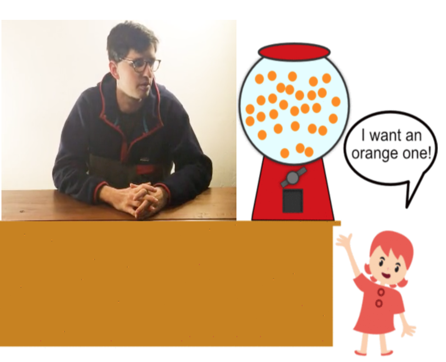
\includegraphics[scale=0.55]{male-condition.png}
\end{center}

\subsection{Procedure}
The number of times participants heard the three utterances and the types of scenes (i.e. the percentages of blue gumballs) varied across the two conditions. In each of the two conditions, there was either a female speaker or a male speaker. Participants in the probably-biased conditions saw 10 exposures with probably for 90\% blue, 5 exposures without modal for 100\% blue (bare form), and 5 exposures with might for 25\% blue (fillers). Participants in the bare-biased condition saw 10 exposures with bare for 90\% blue, 5 exposures with probably for 60\% blue, and 5 exposures with might for 25\% blue. 
After the exposure phase, the participants did the rating task. There were 40 participants in each condition. 


After the exposure phase, participants did the same rating task as in the pre-test experiment. There were 40 participants in each condition.

\subsection{Exclusions}
Catch trials were included to ensure that participants were attending to the task. Catch trials were implemented by putting a gray cross appeared at a random location in the scene. After the scene was completed and before the next scene was shown, participants were asked if they had seen a gray cross in the previous scene. I excluded participants who provided the incorrect answer to more than 25\% of the catch trials (i.e. participants who provide the correct answer less than 12/15 catch trials).


\subsubsection{Results}

The following graphs show the aggregated post-exposure ratings in the two conditions. There are four graphs to show the conditions with a different gendered speaker. Condition 0 was a probably-biased condition with a female speaker, condition 1 was a bare-biased condition with a female speaker, condition 2 was a probably-biased condition with a male speaker, and condition 3 was a bare-biased condition with a female speaker. 


\begin{center}
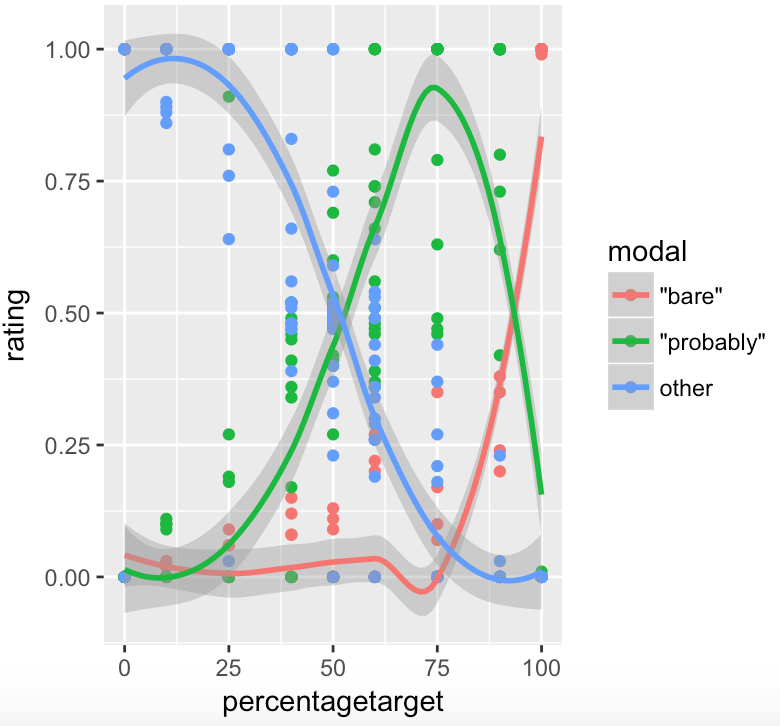
\includegraphics[scale=0.45]{Condition-0-batch1-trials.png}
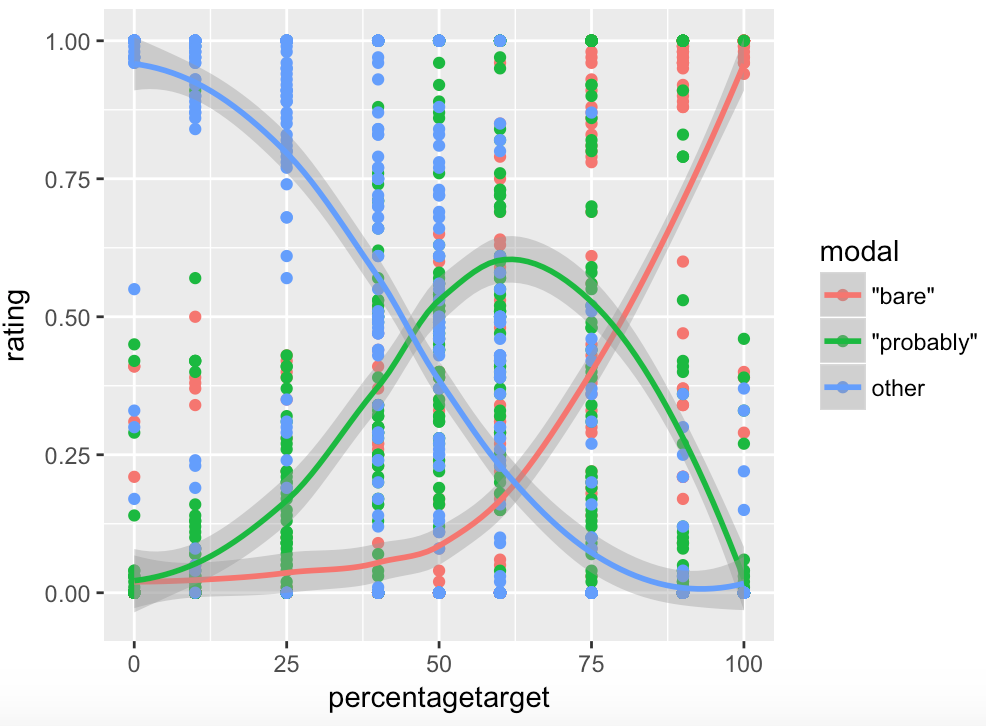
\includegraphics[scale=0.4]{Condition-1-trials.png}
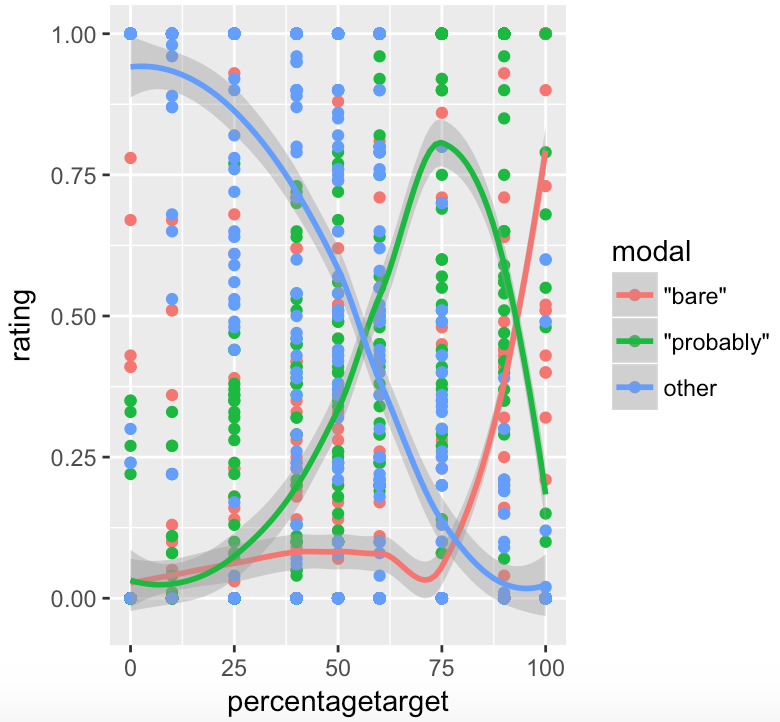
\includegraphics[scale=0.5]{Condition-2-trials.png}
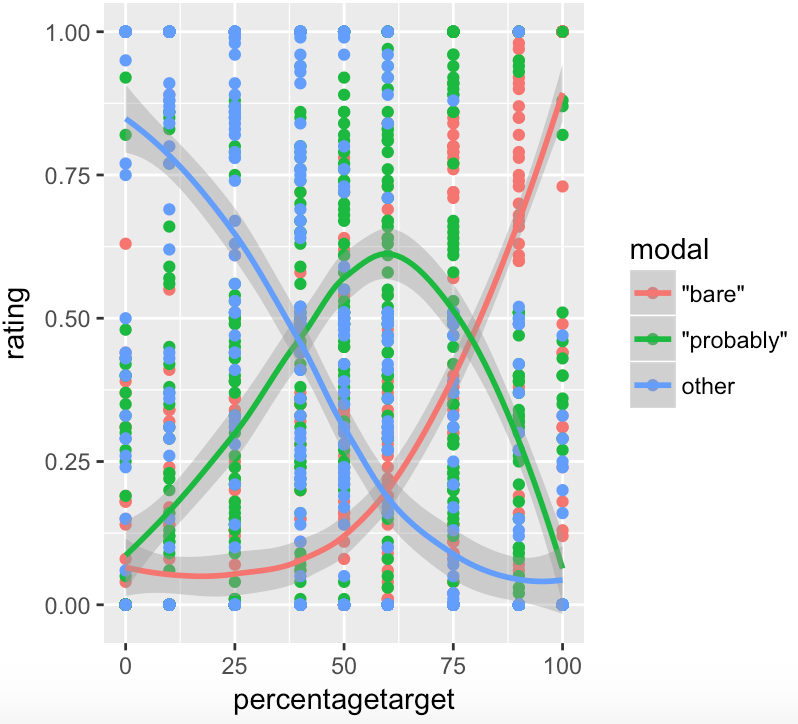
\includegraphics[scale=0.45]{Condition-3-trials.png}

\vspace{2em}
\end{center}
As these graphs show, participants gave high ratings for probably for a larger range of event probabilities in the probably-biased conditions than participants did in the bare-biased condition. The maximally ambiguous point (where a scene was maximally ambiguous as to whether a speaker would use probably or the bare form) in the pre-test experiment was at 85\% of blue gumballs. Listeners’ ratings of probably pushed the maximally ambiguous point to 90\%, showing that the participants picked up on the use of probably and adjusted their speaker expectations appropriately. Contrastingly, participants gave high ratings for the bare expression for a larger range of event probabilities in the bare-biased conditions than participants did in the probably-biased condition. I expected the ratings for the bare form to shift to the left, and the results show that listeners began to increase ratings of the bare form at 80\%, before the maximally ambiguous point of 85\%. 

These results are similar to Schuster’s findings. Schuster studied the uncertainty expressions might and probably, where the maximally ambiguous point for these expressions was when the gumballs were 60\% blue. His results showed that in the probably-biased condition, the listeners’ ratings of probably began to increase before 60\% blue, which caused the maximally ambiguous point to shift to the right. In the might-biased condition, the listeners’ ratings of might continued to increase after 60\% blue, which caused the maximally ambiguous point to shift to the left. My results produced the same shift and revealed how listeners do adapt to a speaker’s use of uncertainty expressions. Additionally, in both studies, there was no effect of gender of the speaker on the listeners’ adaptation. 

\subsection{Discussion}
I wanted to see how listeners use a speaker’s behaviours to predict the probability of their speech. The results show that 20 exposure trials were able to induce adaptation to a speaker’s preference of an uncertainty expression. The results were almost an identical replication to the original results of Schuster. It was very interesting to see how listeners also adapt to speakers when they do not use an uncertainty expression (bare expression). Since I was able to replicate Schuster’s experiment exactly the way he did, it was not surprising to see that the results followed the same pattern. The results show that there is no difference of how strong a listener adapts to different uncertainty expressions; listeners have the ability to remember a speaker’s preference to an uncertainty expression and are capable of using this information to guide predictions. To further these findings, it would be fascinating to continue to test all 15 conditions where there is a different pair of uncertainty expressions used. 

It is also interesting to note the idea of reliability in this study. Since I looked at the bare-form, how does this affect the reliability of a speaker? If a speaker is saying, "you'll get a blue one," when not all the gumballs are blue, this statement is not entirely reliable. If there is a chance that they might not get a blue gumball, we should expect that the speaker should use an uncertainty expression to account for the possibility of not getting a blue gumball. If we hear, "you'll get a blue one," we should expect that all the gumballs are blue and that there should be not other outcome besides a blue gumball. In future studies, it would be interesting to have listeners rate the reliability of a speaker to see if there is a decrease in reliability in the bare-biased condition. 

\newpage\subsection{References}

\begin{indent}Schuster, S., Degen, J. (2018, April 09). Listener adaptation to speaker variation in use of uncertainty expressions. Retrieved from https://github.com/sebschu/adaptation
\end{indent}

Yildirim, I., Degen, J., Tanenhaus, M.K., Jaeger, T. F. (2016, April 01). Talker-specificity and adaptation in quantifier interpretation. Retrieved from \url{https://www.ncbi.nlm.nih.gov/pmc/articles/PMC4742339/}

\printbibliography
%\bibliography{qp-references}


%=====================================================================

%\begin{addresses}
 % \begin{address}
%    Author1 \\
%    Street \\
%    \ldots \\
%    \email{author1@email}
%  \end{address}
%  \begin{address}
 %   Author2 \\
 %   Street \\
 %   \ldots \\
 %   \email{author2@email}
 % \end{address}
 % ...
%\end{addresses}

%=====================================================================

\end{document}
